\documentclass[hidelinks,12pt,a4paper]{article}
\usepackage[italian]{babel}
\usepackage[utf8]{inputenc}
\usepackage{fourier} 

% To avoid GitHub Action error
\usepackage{hyperref}

% Images
\usepackage{graphicx}
\usepackage{caption}
\usepackage{subcaption}
\usepackage{float}
\graphicspath{ {../Images} }

% Stop hyphenation
\usepackage[none]{hyphenat}

% To draw over images
\usepackage{tikz}

% Adjust paragraph.
\usepackage{changepage}
\usepackage{geometry}

% License
\usepackage[
type={CC},
modifier={by-nc-sa},
version={4.0},
]{doclicense}

% Command to create fake sections
\newcommand{\fakesection}[1]{%
	\par\refstepcounter{section}% Increase section counter
	\sectionmark{#1}% Add section mark (header)
	\addcontentsline{toc}{section}{\protect\numberline{\thesection}#1}% Add section to ToC
}

% Defining enviroment and commands to write puzzle weaves over images
\pgfmathparse{int(random(1,120))}

\newcommand{\side}[1]{
	(0.0,#1*0.00) .. controls (0.0,#1*0.00) and (0.4,#1*-0.04) .. 
	(0.4,#1*0.04) .. controls (0.4,#1*0.11) and (0.2,#1*0.26) .. 
	(0.5,#1*0.26) .. controls (0.8,#1*0.26) and (0.6,#1*0.11) .. 
	(0.6,#1*0.04) .. controls (0.6,#1*-0.04) and (1.0,#1*0.00) .. 
	(1.0,#1*0.00)
}

\newcommand{\piece}[2]{
	\draw[ultra thick] \side{#1} [rotate around={90:(0.5,0.5)}] \side{#2};
}

\pgfmathdeclarerandomlist{inout}{{-1}{1}}

%Defining Command to write jigsaws over an image
\newcommand{\puzzle}[4]{  % Argument 1 -> includegraphics entire string
												  % Argument 2  -> define Xmax (jigsaw pieces)
												  % Argument 3 -> define Ymax (jigsaw pieces)
												  % Argument 4 ->  Image caption

\begin{minipage}{\linewidth}
	\centering
	\begin{tikzpicture}
		
		\node[anchor=south west,inner sep=0] (image) at (0,0) {#1};
		
		\def\xmax{#2}
		\def\ymax{#3}
		
		
		\foreach \x in {0,...,\xmax}{
			\foreach \y in {0,...,\ymax}{
				
				\ifnum\y=0
				\def\bottom{0}
				\else
				\pgfmathrandomitem{\bottom}{inout}%
				\fi	
				
				\ifnum\x=\xmax
				\def\right{0}
				\else
				\pgfmathrandomitem{\right}{inout}%
				\fi
				
				\begin{scope}[xshift=\x cm, yshift=\y cm]
					\piece{\bottom}{\right}
				\end{scope}
			}
		}
		
		\draw (0,0) -- (0,\ymax+1) -- (\xmax+1,\ymax+1);
		
	\end{tikzpicture}
\end{minipage}

\vspace*{\fill}
\centering
\fboxrule=2pt{
	\fbox
	{
		\begin{minipage}{0.95\linewidth}
			\centering
			#4
		\end{minipage}
}}
\newpage

}

\begin{document}
	
	\title{\textbf{\centering{Laboratorio creativo per bambini}\\Puzzle sulle opere d'arte}}
	\author{Alice Balestieri\\Francesco Rombaldoni}
	\date{}
	
	\maketitle
	\newpage
	
	\tableofcontents
	\newpage
	
	\section{Come giocare}
	\begin{center}
		\textbf{Le regole sono rivolte agli operatori.}
	\end{center}
	
	\subsection{Variante 1}
	Dopo aver stampato su del cartoncino e ritagliato i vari puzzle, mischiare i vari pezzi di tutti i puzzle ritagliati (per esempio mettendoli in una scatola per poi scuoterla), per poi disporli casualmente su di un tavolo. I bambini dovranno risolvere i vari puzzle riconoscendo i vari pezzi delle opere.\\
	Quando i bambini hanno finito di risolvere i puzzle, domandargli se si ricordano i nomi delle opere che hanno ricomposto.
	
	\subsection{Variante 2}
	Dopo aver stampato su del cartoncino e ritagliato i vari puzzle, mischiare i vari pezzi di tutti i puzzle ritagliati (per esempio mettendoli in una scatola per poi scuoterla), per poi disporli casualmente al centro di un tavolo. Dividere i bambini in squadre di massimo tre elementi, successivamente assegnare ad ogni squadra due opere prese dalla lista delle opere trasformate in puzzle. I bambini dovranno cercare i vari pezzi dell'opera che devono ricomporre per poi risolvere i puzzle sui bordi del tavolo (queste due azioni possono essere fatte simultaneamente dai vari elementi del gruppo).
	
	\section{Lista delle opere trasformate in puzzle}
	\begin{itemize}
		\item Mengaroni Ferruccio - Medusa
		\item Bellini Giovanni - Incoronazione della Vergine
		\item Vitale da Bologna - Sant'Ambrogio in trono
		\item Desani Pietro - Rebecca ed Eleazar
		\item Leda e il Cigno (Giove) di fattura ad opera di Giovanni Antonio Garella
		\item Stipo con vedute di Roma
		\item Orologio notturno
		\item Scacciani Antonio - Vassoio - Rosa
		\item Milani Aureliano - Mercato
		\item Berentz Christian - Fiori e frutta con bicchieri di cristallo
		\item Gianlisi Antonio Junior - Trompe l'oeil con sonetto in onore di Eugenio di Savoia e mensola con oggetti
		\item Gianlisi Antonio Junior - Trompe l'oeil con paesaggio forbici e mensola con oggetti
		\item Realfonzo Tommaso - Natura morta con dolci frutta uova e formaggi
		\item Gessi Giovan Francesco - Morte di Adone
	\end{itemize}

	\newgeometry{top=15mm, bottom=15mm}
	\begin{adjustwidth}{-30mm}{-30mm}
		
		\fakesection{Puzzle}
	
		\centering{\Large \textbf{Puzzle}}
		\vspace{5mm}
		
	
	
	% Start inserting images (used images formats from "Coloring_Artworks")
	
			
		\puzzle{\includegraphics[scale=3.6]{Mengaroni_Ferruccio-Medusa.jpg}}{18}{18}{Mengaroni Ferruccio - Medusa.}
			
		\puzzle{\includegraphics[scale=0.201]{Bellini_Giovanni-Incoronazione_della_Vergine.jpg}}{14}{23}{Bellini Giovanni - Incoronazione della Vergine.}
		
		\puzzle{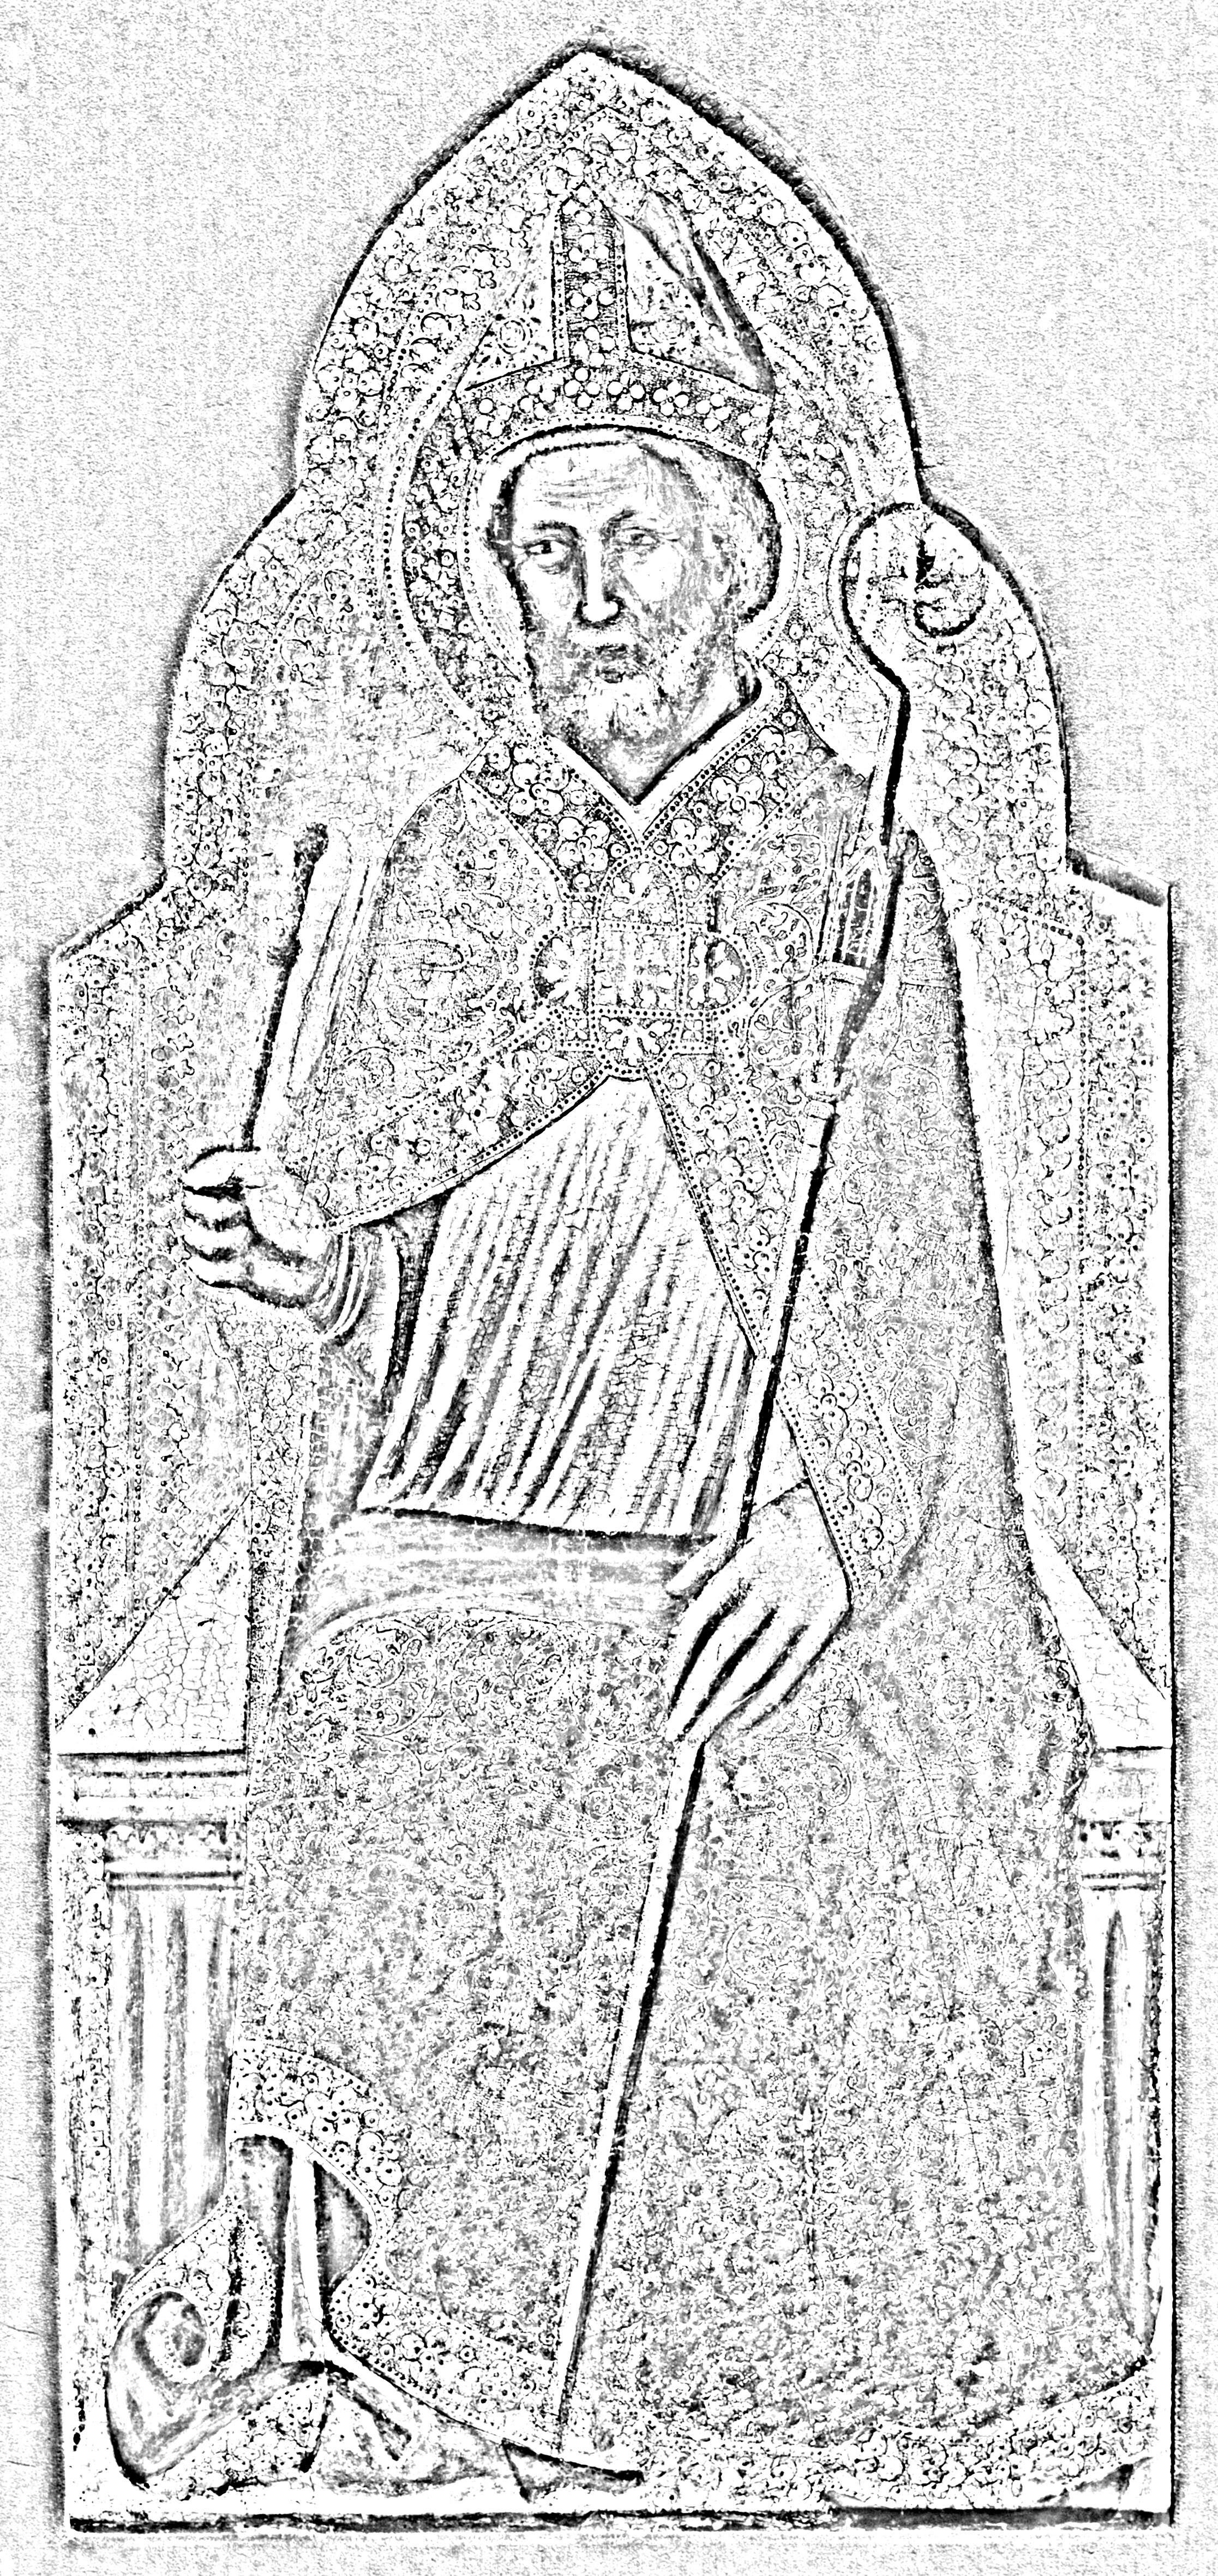
\includegraphics[scale=0.14]{Vitale_da_Bologna-Santo_Ambrogio_in_trono.jpg}}{10}{23}{Vitale da Bologna - Sant'Ambrogio in trono.}
		
		\puzzle{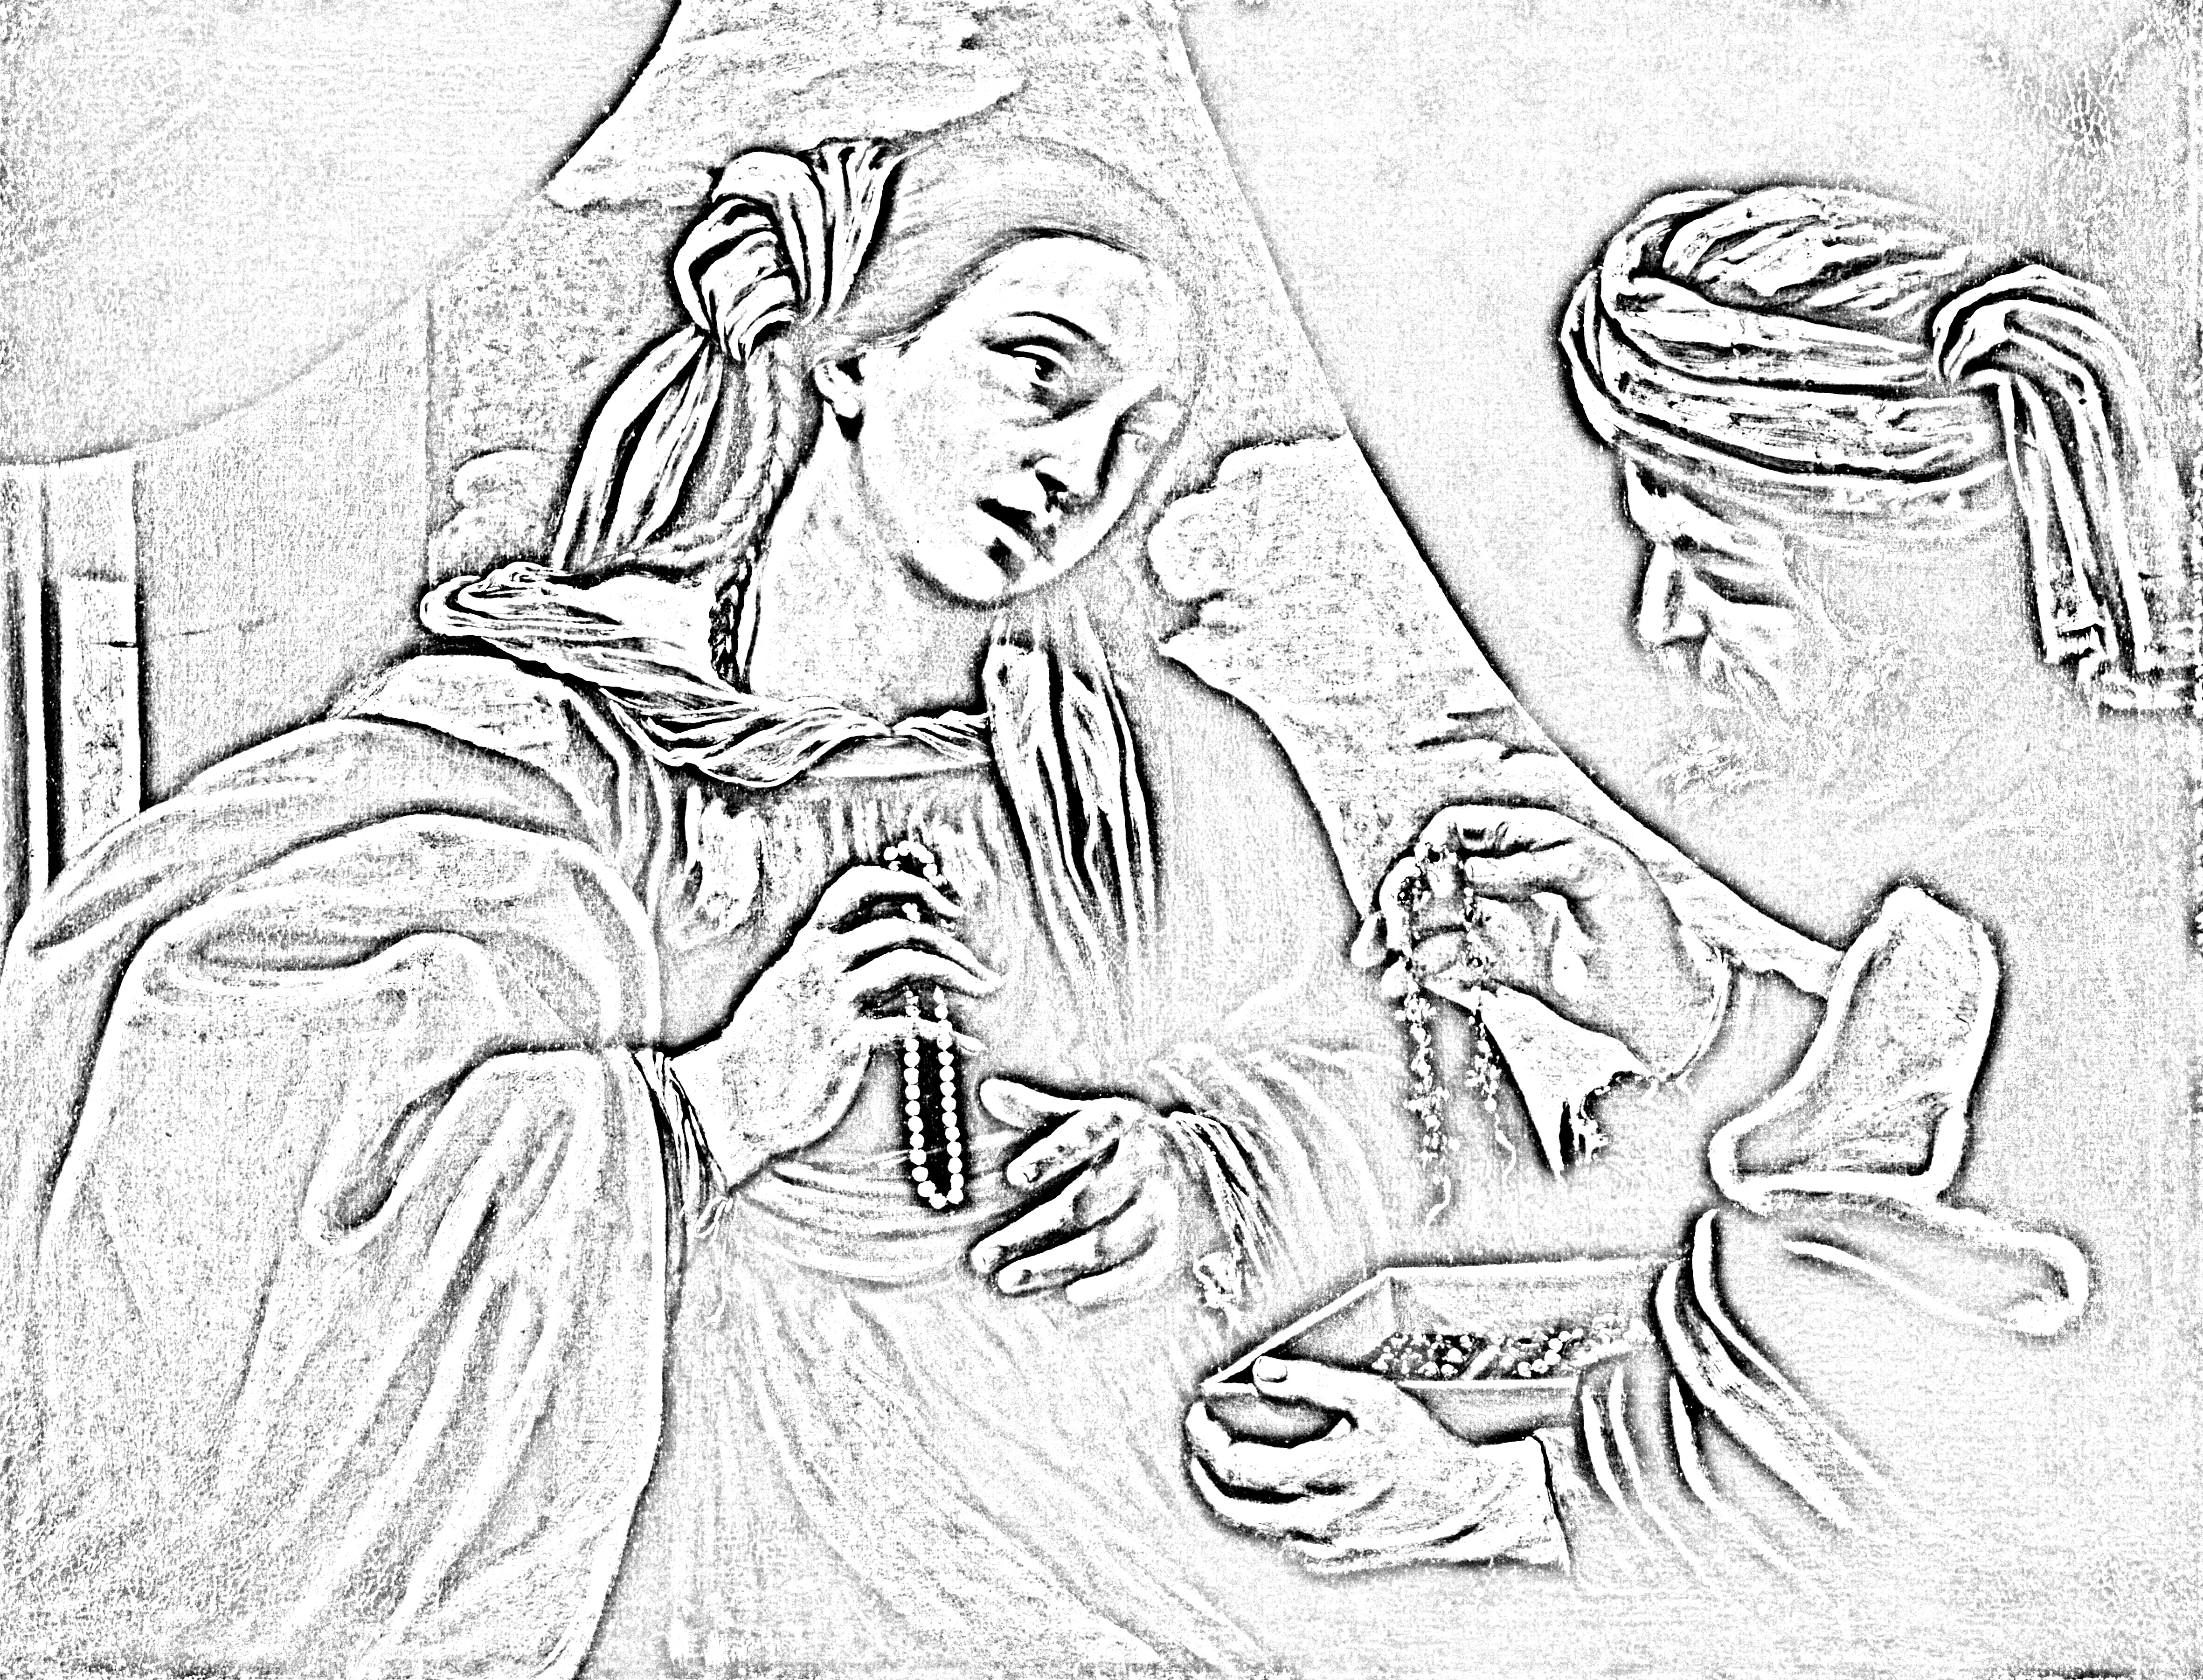
\includegraphics[scale=0.11]{Desani_Pietro-Rebecca_ed_Eleazar.jpg}}{17}{13}{Desani Pietro - Rebecca ed Eleazar.}
		
		\puzzle{\includegraphics[scale=3.78]{Giovanni_Antonio_Garella-Leda_e_il_cigno.jpg}}{19}{19}{Giovanni Antonio Garella - Leda e il Cigno.}
		
		\puzzle{\includegraphics[scale=0.886]{Vedute_di_Roma_1.jpg}}{17}{10}{Stipo con vedute di Roma.}
		
		\puzzle{\includegraphics[scale=0.61]{Orologio_notturno.jpg}}{15}{21}{Orologio notturno.}
		
		\puzzle{\includegraphics[scale=2]{Scacciani_Antonio-Vassoio-Rosa.jpg}}{16}{12}{Scacciani Antonio - Vassoio - Rosa.}
		
		\puzzle{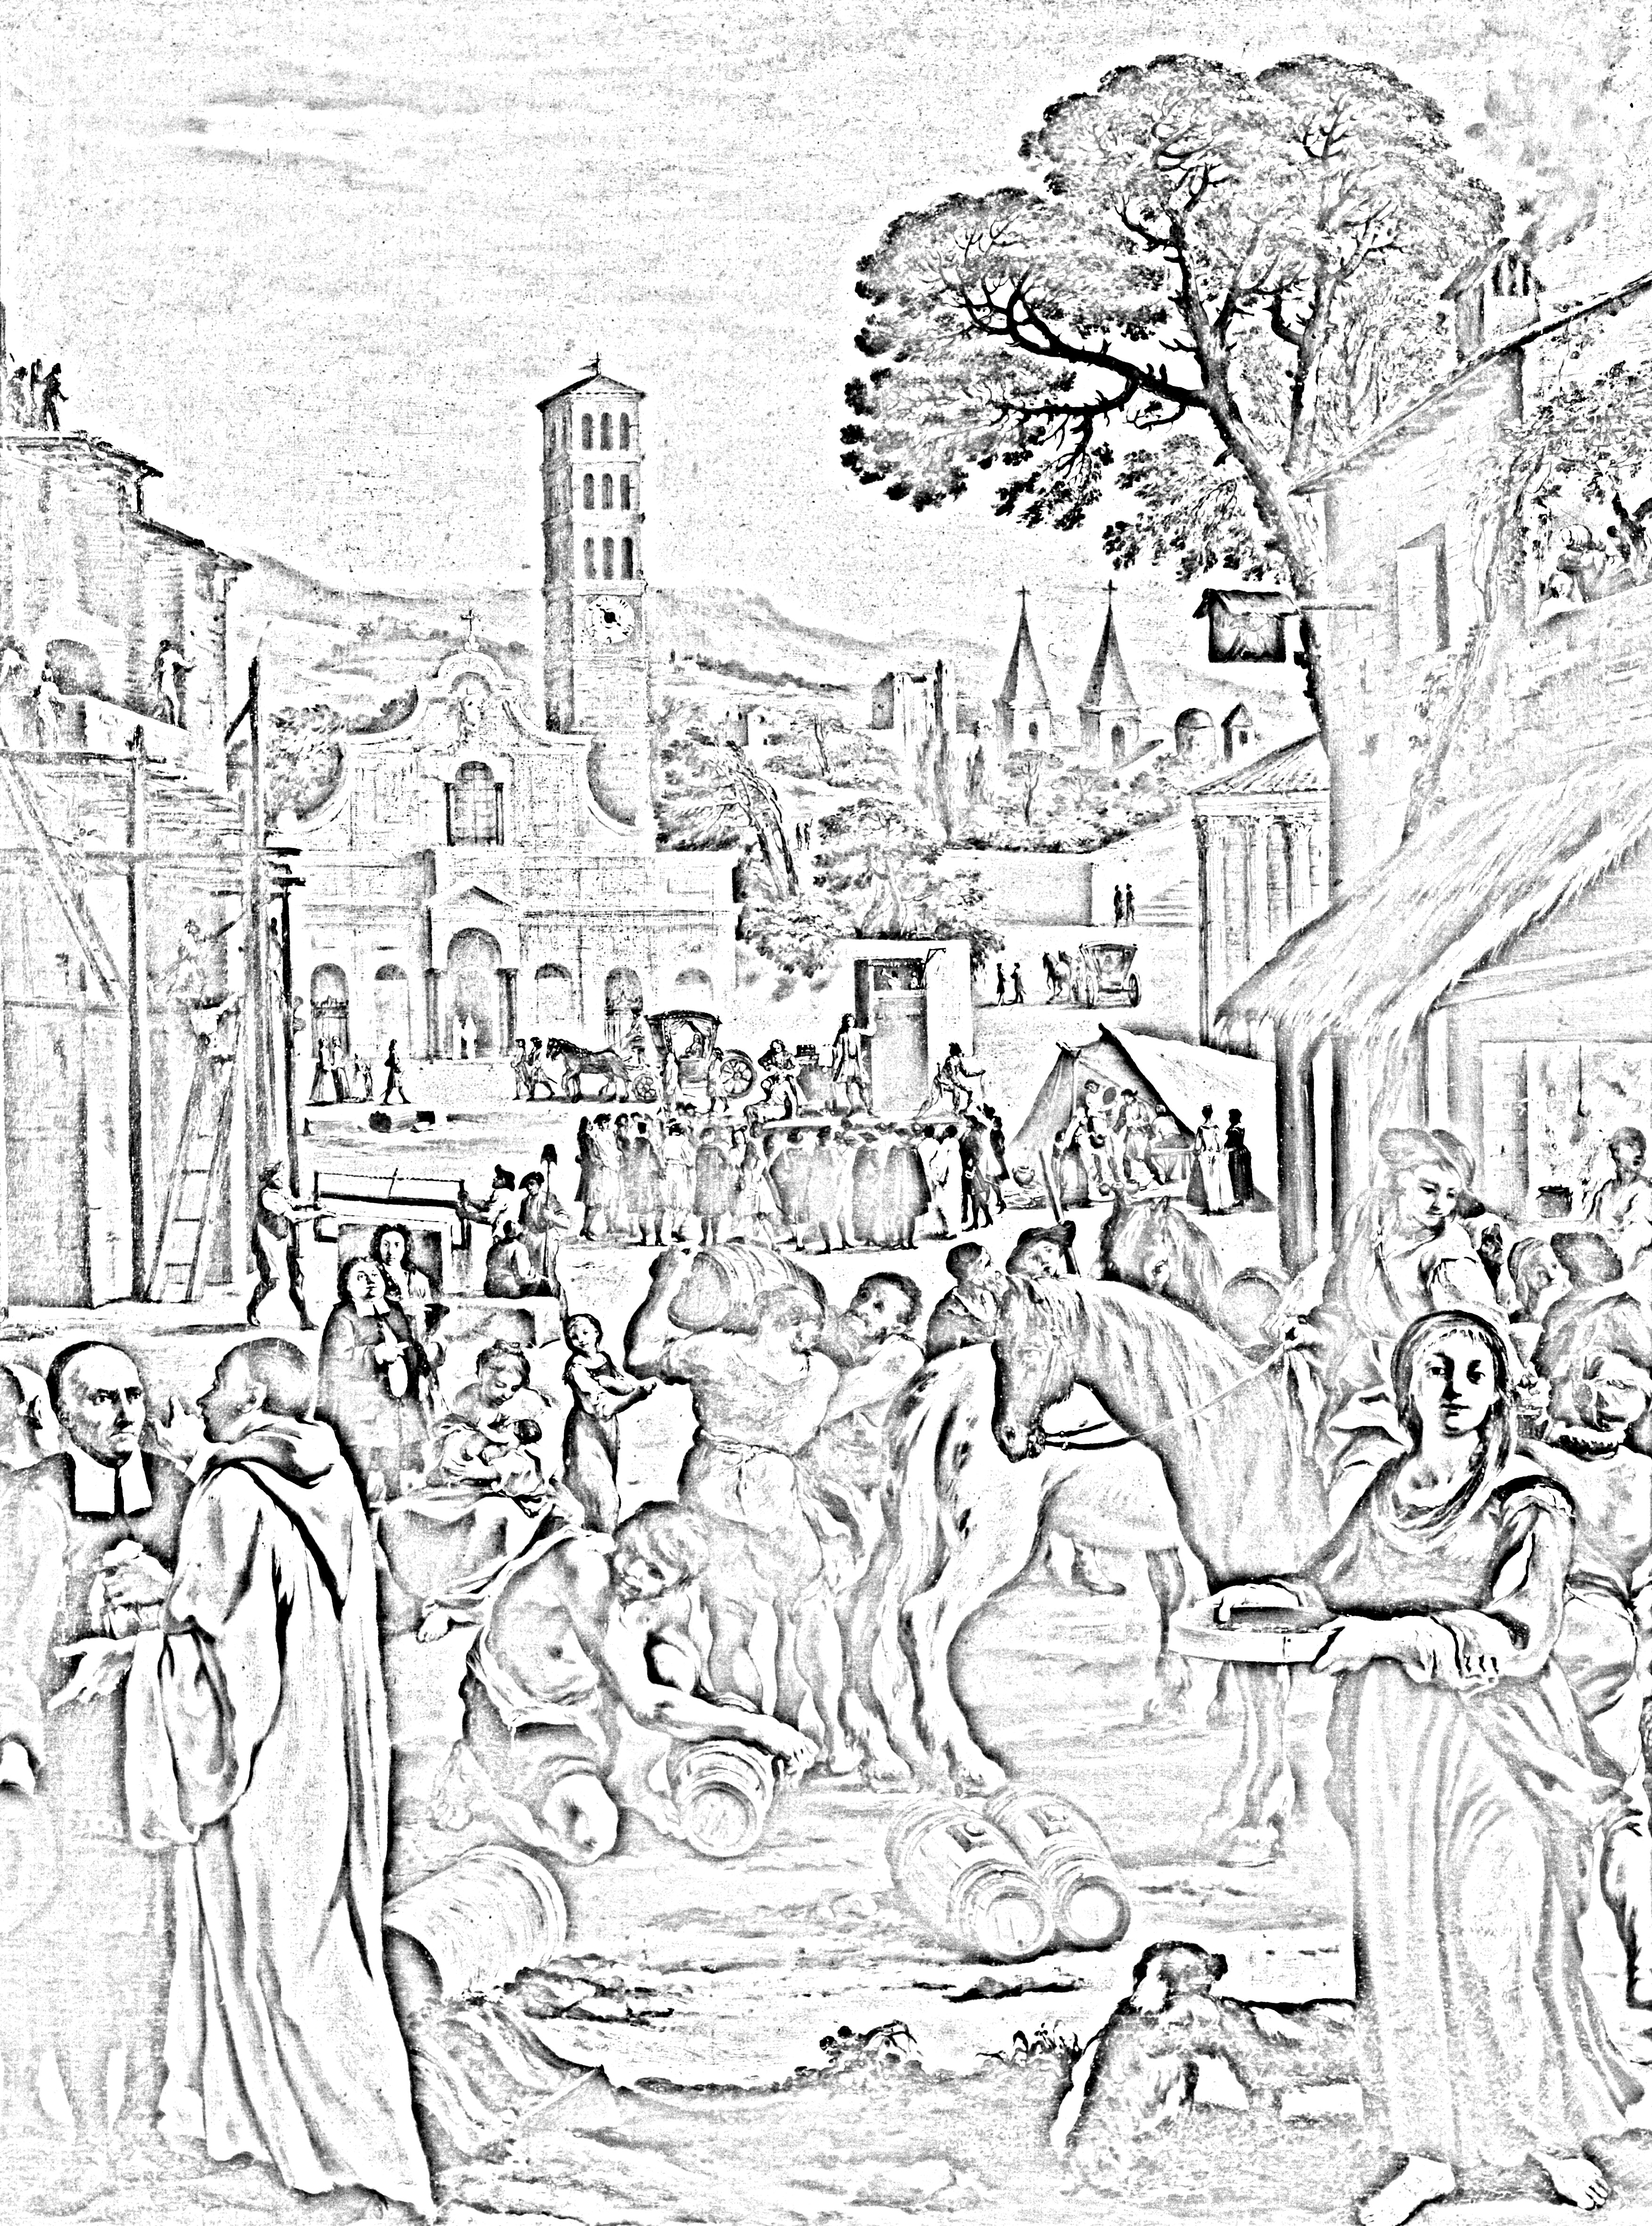
\includegraphics[scale=0.13]{Milani_Aureliano-Mercato.jpg}}{15}{21}{Milani Aureliano - Mercato.}
		
		\puzzle{\includegraphics[scale=0.2]{Berentz_Christian-Fiori_e_frutta_con_bicchieri_di_cristallo.jpg}}{16}{22}{Berentz Christian - Fiori e frutta con bicchieri di cristallo.}
		
		\puzzle{\includegraphics[scale=0.2]{Gianlisi_Antonio_Junior-Trompe_l_oeil_con_sonetto_in_onore_di_Eugenio_di_Savoia_e_mensola_con_oggetti.jpg}}{15}{21}{Gianlisi Antonio Junior - Trompe l'oeil con sonetto in onore di Eugenio di Savoia e mensola con oggetti.}
		
		\puzzle{\includegraphics[scale=0.202]{Gianlisi_Antonio_Junior-Trompe_l_oeil_con_paesaggio_forbici_e_mensola_con_oggetti.jpg}}{16}{22}{Gianlisi Antonio Junior - Trompe l'oeil con paesaggio forbici e mensola con oggetti.}
		
		\puzzle{\includegraphics[scale=1.8]{Realfonzo_Tommaso-Natura_morta_con_dolci_frutta_uova_e_formaggi.jpg}}{19}{13}{Realfonzo Tommaso - Natura morta con dolci frutta uova e formaggi.}
		
		\puzzle{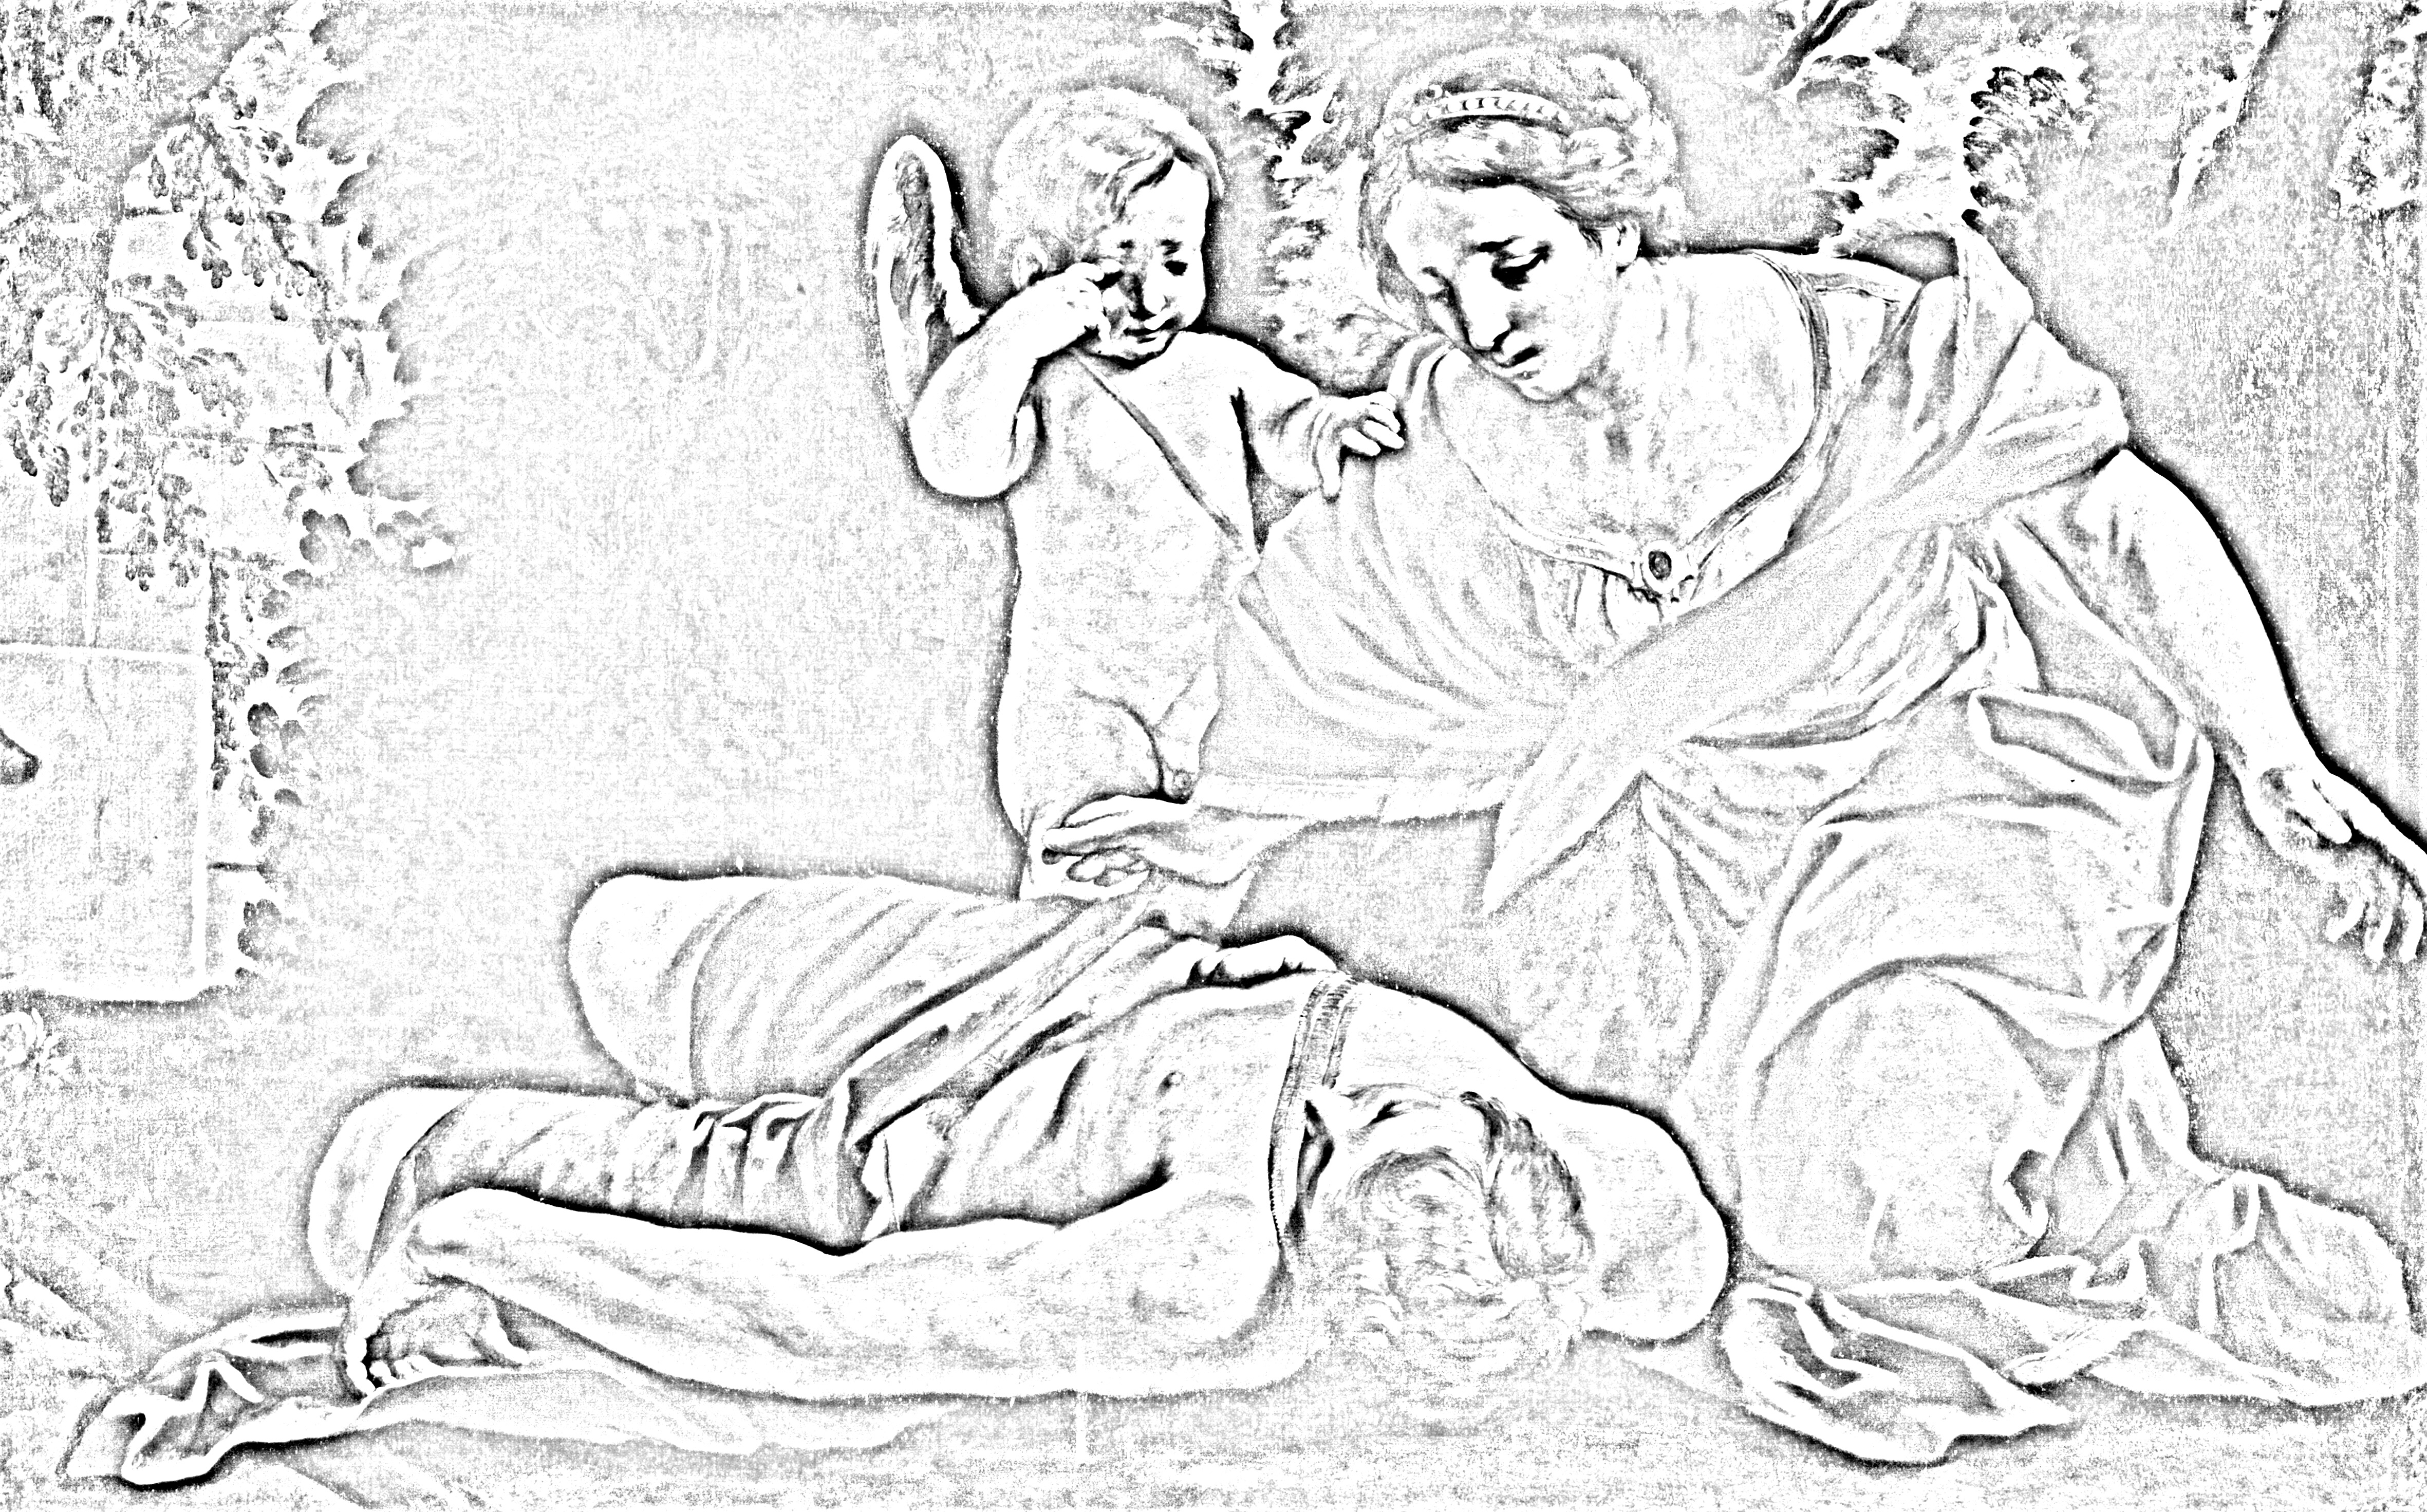
\includegraphics[scale=0.114]{Gessi_Giovan_Francesco-Morte_di_Adone.jpg}}{18}{11}{Gessi Giovan Francesco - Morte di Adone.}
	
		\vspace*{\fill}
		% Print license shield
		\doclicenseThis
	
	\end{adjustwidth}
\end{document}
